\documentclass[pdftex,12pt,a4paper]{article}

\usepackage[french]{babel}
\usepackage[utf8]{inputenc}
\usepackage[T1]{fontenc}

\usepackage[final]{pdfpages}
\usepackage{fullpage}

\usepackage{url}
\usepackage{graphicx}

\newcommand{\HRule}{\rule{\linewidth}{0.5mm}}
\newcommand{\jasmed}{\texttt{JaSMEd}}

\begin{document}

\begin{titlepage}

\begin{center}


\includegraphics[height=3cm]{./logo_upmc.png} \\[0.8cm]

\textsc{\LARGE Rapport de Projet}\\[1.5cm]

\HRule \\[0.4cm]
{\huge JaSMEd}\\[0.4cm]
{ \huge \bfseries JavaScript Music Editor}\\[0.4cm]

\HRule \\[1.5cm]

\begin{minipage}{0.4\textwidth}
\begin{flushleft} \large
\emph{Etudiants:}\\
Cl�ment \textsc{Bossut}\\
Valentin \textsc{Cassat}\\
Jaime \textsc{Chao}\\
Thibaud \textsc{Cummings}\\
\end{flushleft}
\end{minipage}
\begin{minipage}{0.4\textwidth}
\begin{flushright} \large
\emph{Encadrant:} \\
Emmanuel \textsc{Saint-James}\\
\end{flushright}
\end{minipage}\\[4 cm]

\large
Parcours SAR\\
Universit� Pierre et Marie Curie\\
UPMC Paris\\

\vfill
M1 - S2 - 2012
%{\large \today}

\end{center}

\end{titlepage}



\begin{center}
{\huge \bfseries Sujet}\\[1.5cm]
\end{center}
{\Large \bfseries Editeur musical collaboratif en JavaScript}

\bigskip
La nouvelle interface WebSocket permet d’utiliser les navigateurs pour implémenter facilement en JavaScript des applications collaboratives et interactives. Ajoutée à la nouvelle interface WebAudio, on peut en particulier concevoir un éditeur de pistes musicales affiché par un navigateur Web standard, sur lequel opère à la fois l’utilisateur du navigateur et ses correspondants.\\
Le but du projet est de développer un tel éditeur, en traitant en particulier les problèmes d’accès concurrents à une même partie des pistes musicales éditées collaborativement. Se pose aussi la question de l’archivage sur le serveur des différents états de la partition, et la manière d’y accéder.\\
La question des protocoles audio à utiliser sera aussi abordée.

\vfill

\pagebreak

\tableofcontents

\pagebreak

\section{Introduction}

Nous avons proposé \jasmed\ car il s'inscrit à la fois dans le domaine des applications réparties, et reflète nos orientations musicales dans la pratique de l'informatique.
C'est dans un cadre internet en constante transformation que l'on a développé \jasmed, une application client/serveur qui tire partie des nouvelles API d’HTML5.

\medskip
\jasmed\ est un éditeur musical multi-utilisateur temps réel implémenté à partir des nouveaux standards du web qui tire sa spécificité de part son approche de composition polyrythmique\footnote{Superposition de plusieurs parties ayant chacune un rythme différent et dont les accents d'appui ne coïncident pas entre eux (Larousse de la Musique, Paris, t. 2, 1982, p. 1247).}.\\
Actuellement il n'existe pas d'outils pour créer une polyrythmie musicale de manière collaborative. En général il n'y a pas de moyens simples permettant d'écrire ce genre de rythmes complexes, et encore moins sur internet où la majeure partie des applications musicales ne sont pas de véritables outils de composition.\\
C'est en faisant ce constat que nous est apparue l'idée de développer \jasmed.
De part son approche de l'édition web collaborative, notre travail s'inscrit parfaitement dans le cadre du master SAR\footnote{Systèmes et Applications Répartis}.\\
Il faut préciser que c'est une application non encore aboutie que nous présentons ici, elle est fonctionnelle mais mais ne représente pas encore complètement l'ampleur du projet.

\section{État de l'art}

Le HTML est le langage principal du World Wide Web, le W3C\footnote{World Wide Web Consortium} est actuellement en train de travailler sur HTML5, qui est la 5ème révision majeure de ce langage. Il est important de noter que cette version est toujours à l'état d'ébauche\footnote{\url{http://www.w3.org/TR/html5/index.html}} et ne cesse d'évoluer.
HTML5 fournit une flopée de nouvelles API, notamment la balise <audio>\footnote{\url{http://www.whatwg.org/specs/web-apps/current-work/multipage/the-video-element.html#the-audio-element}} qui permet de fournir un lecteur audio simple, et enfin de se passer des vieux lecteurs et codecs lourds et privés (Windows media player, realPlayer, quicktime).
Malheureusement ce n'est pas suffisant pour un traitement de l'audio plus poussé, c'est ainsi que des librairies audio ont fait leur apparition.

\medskip
Les navigateurs Firefox et Google Chrome ont ainsi développé leur propre API audio, permettant de véritablement traiter le signal numérique sur nos navigateurs.
Ces API ont été crées dans le but d'offrir au web game developer un vrai environnement sonore pour la conception de jeu sur le web, dans la synergie avec la sortie du WebGL.\\
WebAudio est un peu plus poussée que Firefox, de même elle bénéficie d'un plus grand engouement dans la communauté web. D'après les listes de diffusion du working draft du W3C, l'API de Google serait même candidate à une standardisation imminente.

WebAudio, largement inspiré du sytème CoreAudio d'Apple, pour Google Chrome
Audio Data Api pour firefox

\medskip
Il existe déjà beaucoup de librairies javascript qui abstraient ces API et permettent de construire des applications audio sur le web plus facilement\footnote{\url{https://wiki.mozilla.org/Audio_Data_API#JavaScript_Audio_Libraries}}.
Certaines, comme audiolib.jsc{audiolib} ou audionode.js, permettent d'abstraire les différences entre les 2 API concurrentes et ainsi grandement faciliter la portabilité entre navigateurs.\\
Une quantité de nouvelles applications web musicales sont apparues sur la toile avec l'arrivée d'HTML5. La majeure partie de ces applications ont un aspect ludique (ou se bornent à être de simples gadgets) , et ne sont pas vraiment utiles à des compositeurs/musiciens. On en a recensé un échantillon : 
\begin{itemize}
\item jeux sonores
\item éditeur musical
\end{itemize}

Si on regarde les logiciels d'édition musicale ils ne permettent pas de créer facilement des musiques poly-rythmiques, mais se prettent plus facilement à composer des tempos binaires. Les plus connus d'entre eux :\\
Ableton Live\\
\url{http://harmonyseq.wordpress.com/}\\
\url{http://www.technitone.com/#}

\medskip
Notre projet s'inscrit donc au coeur des avancées actuelles du web dans le domaine de l'audio, et il propose une vision d'édition poly-rythmique peu répandue dans les logiciels audio.


\section{Conception}

Avant de nous lancer dans l’implémentation de l’application nous avons longuement réfléchis à une conception efficace du problème car nous le savions complexe. Nous voulions un application dont la prise en main soit facile, qui soit performante et innovatrice, et enfin qui puisse être facilement améliorée par la suite.\\
Nous décrivons ici les trois grands axes de réflexion qui nous ont permis de démarrer l’application sur de bonnes bases.

\subsection{Structures}

L’application a été séparée en deux parties distinctes que sont l’affichage et la lecture du son. Ceci pour des raisons de performances, car la structure optimale pour l’affichage ne l’est pas pour la lecture du son et inversement. Nous avons ainsi pu nous partager le travail aisément.

L'idée est de se détacher des notations solfégiques usuelles pour s'orienter vers une écriture musicale plus ludique et intuitive, adaptée notamment aux enfants. Dans ce but, nous nous sommes émancipé de la signature rythmique et avons imaginé une division en blocs (aparentable à des mesures). Tous les blocs ont une durée identique, et sont indépendamment subdivisibles (un bloc s'apparente à une mesure avec une signature et une vitesse d'exécution adapté).

\subsubsection{Musicale}

I’ll do it

Ci-dessous est décrit un choix d’implémentation si je ne me trompe !
comment stocker l’information musicale.
-> options envisagées: OSC, MIDI, (structure propriétaire)
OSC: qu’un protocole, ne présente aucune manière pré-définie de stocker de l’information musicale.
MIDI: le MIDIFile est standard pour ça mais pose plusieurs problèmes: changer de rythme implique ‘hacker’ le midi tempo qui est exprimé en nb de mmsec dans une noire...
+ le fait que la plupart des logiciels utilisent le MIDI en mode ‘non compatible justement... donc inutile.. (plus du tout ‘portable’)
à partir de ça, expliquer la structure, ‘blocs’, abstraction de notation musicale... pourquoi les couches etc...

\subsubsection{Visuelle}

Pour ce qui concerne le rendu graphique de l’application, il est intéressant de séparer la vue des données, à la manière d’une architecture MVC. Une fois la vue correctement liée au changement des modèles, on ne s’occupe plus qu’à la modification des données et la vue suit. De plus ceci a un avantage dans la réutilisation du code côté serveur comme nous le verront dans la section archivage.
Les structure des données de l’affichage est en quelque sorte conditionnée par les possibilités du couple HTML5/CSS3.
/** parler des blocs, calques, notes, … ? */

\subsection{Collaboration}

Un point innovant du projet et qui justifie l’utilisation de technologies récentes, est la collaboration temps réel entre plusieurs client. Le choix de développer l’application dans un navigateur web peut paraître restrictif à première vue, mais il apporte une plus grande facilité de développement pour son aspect collaboratif.
En effet, le nouveau protocole WebSocket permet de faire communiquer le navigateur web du client et le serveur web de manière bi-directionnelle et full-duplex, ce qui est alors indispensable pour répercuter les changements d’un client à l’autre dans un lapse de temps raisonnable. Ainsi toute modification locale apportée à l’éditeur par un client est envoyée au serveur, qui à son tour broadcast l’information aux autres clients.
Seulement cette synchronisation introduit différents problèmes dont voici une analyse.

\subsubsection{Concurrence}

comment assuré une concurrence cohérente (mode musique...)
-> lock + duplication de piste. <= de la folie à mon avis.
On peut peut-être dire qu’on est pas d’accord et que ça reste à débattre... :P

Il faut parler des locks ici à mon avis.
Et Valentin, if you don’t mind, je changerais tous tes “sélections” en “notes”.
Tu parles dans le code ou dans le rapport?
La différenciation sémantique que je fais, c’est que avant que la note soit intégré à la structure c’est une “sélection” et une fois qu’elle peut être lu par le player, c’est une “note”. selection c’est plus parlant pour l’interface graphique en effet... c’est limite mieux de distinguer les deux... enfin je ne pense pas que grizix parlait de changer ça dans le code.

Seule la superposition de sélections simultanées pause un problème de concurrence. (de ce que j’arrive à imaginer).
Sommes nous d’accord sur la solution apportée?
Une solution pourrait être de tester s’il y a superposition au moment de la synchronisation des données sur le serveur. Si une sélection n’est pas possible, le serveur répond au client qui a fait la sélection pour qu’il supprime sa sélection, et ne diffuse pas la sélection aux autres clients. 

\subsubsection{Archivage}

Permettre à un client de se joindre à l’élaboration d’un morceau en cours de route, implique qu’une version synchronisé du morceau peut être récupérée à tout moment sur le serveur. Il faut donc garder une copie des données sur le serveur et les mettre à jour au même moment où le serveur reçois des modifications de la part d’un client.
Pour cela nous pouvons utiliser sur le serveur les deux structures de données (musicale et visuelle) présentes côté client. Elles seront alors maintenues synchronisées de la même manière que celles des clients, à l’aide des messages échangés entre ces derniers. Puis à la connexion d’un nouveau client, ou bien lorsqu’un client souhaitera recharger son application, le serveur pourra exporter le contenu des deux structures, afin que le client puisse initialiser ses structures locales dans le même état que celles du serveur. Il faut alors ajouter des fonctions d’importation et d’exportation de leur contenu aux deux structures. Le fait d’utiliser le même langage (JavaScript) côté serveur et côté client, est ici un avantage, car il permet la réutilisation du code.

L’utilisateur peut ainsi construire un morceau en accolant des blocs et en spécifiant pour chacun le nombre de temps égaux à insérer dans celui-ci. De cette manière, il est possible de reproduire toute construction rythmique (à la manière des constructions LEGO).\\
Un même bloc peut être composé de différents “calques”, un calque représentant ce bloc avec une subdivision particulière : cela permet d’éditer simplement de la polyrythmie.

Est-ce qu’on parle de comment le serveur gère les clients (inscription à une salle, …)?

\subsection{Modularité}

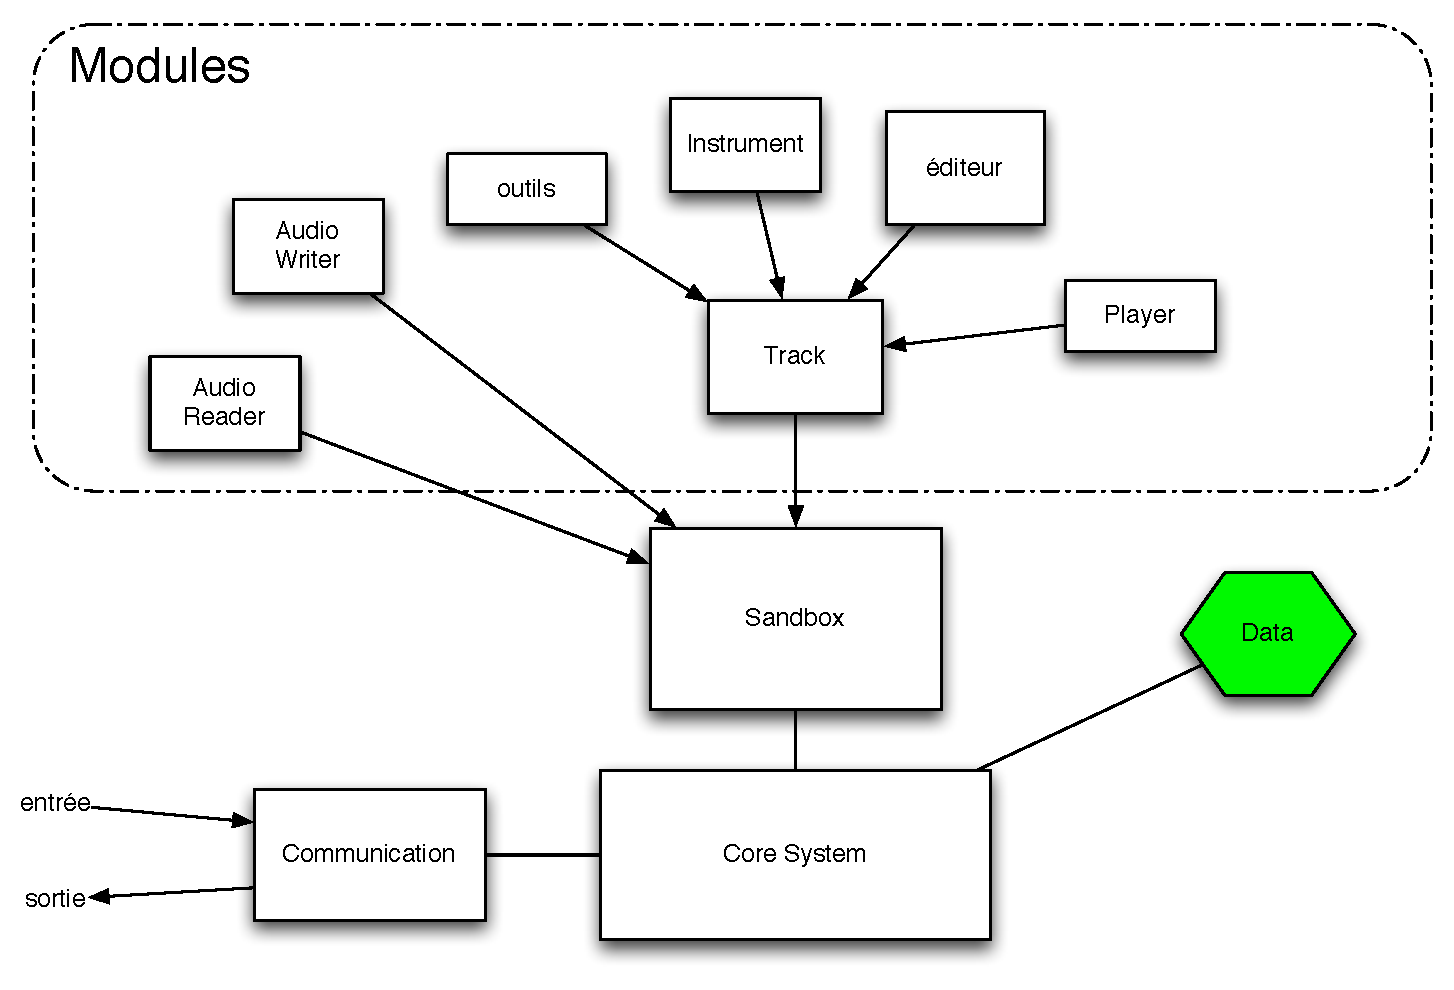
\includegraphics[width=\linewidth]{./PSAR-Client}

L'utilisateur peut ainsi construire un morceau en accolant des blocs et en spécifiant pour chacun le nombre de temps égaux à insérer dans celui-ci. De cette manière, il est possible de reproduire toute construction rythmique (à la manière des constructions LEGO).\\
Un même bloc peut être composé de différents "calques", un calque représentant ce bloc avec une subdivision particulière : cela permet d'éditer simplement de la polyrythmie.

effort de découper en modules indépendants
module de médiateur
pattern MVC
modification et amélioration + simple à l’avenir
pour s’assurer que l’application soit extensible avec un minimum de re-écriture de code... qu’on puisse chacun d’entre nous fonctionner sur des parties indépendantes...
décrire aussi les découplages pertinents: la structure est fortement couplé au player... elles vont ensembles. le fait d’avoir découper les informations sonores (structure) des informations visuelles (backbone) est d’autant plus intéressant qu’il permet d’avoir des représentations différentes du morceaux... potentiellement...

\section{Implémentation}

\subsection{Technologies utilisées}

\subsubsection{Confort de développement}

Une part importante de la réussite d’un projet en équipe réside dans la collaboration entre les membres de l’équipe. C’est pour cela que nous avons tenu dès le début à mettre en place des outils pour faciliter cette collaboration.
Nous avons commencé par partager des Google Docs, afin de fixer les choix aussi bien de conception que d’implémentation, de manière à avoir des documents de référence. Y est répertorié toute la documentation qui nous a aidé au développement de l’application, mais aussi les différents modules qui composent l’application et les messages échangés entre eux.
Ensuite, durant notre documentation, nous avons remarqué que beaucoup de projets open-source que nous utilisons ont un dépôt GitHub pour faire participer la communauté au développement. C’est alors un moyen facile pour nous de mettre en commun le développement de l’application, dans un premier temps entre les membres de l’équipe du projet, mais aussi par la suite à toute autre personne souhaitant participer au projet.
Nous avons alors découvert Git pour la gestion des versions en local, qui s’avère être un outils presque indispensable dans le développement d’une application telle que JaSMEd.
Le code source de JaSMEd est donc disponible sur le dépôt GitHub à l’adresse suivante: https://github.com/Acekat/JaSMEd. Nous avons pris le partie de commenter et rédiger notre code en anglais, afin de permettre au plus grand nombre de participer au projet.

\subsubsection{JavaScript et ses bibliothèques}

\paragraph{JavaScript}
Toutes les librairies que nous avons utilisées, aussi bien du côté client que du côté serveur, sont écrites en JavaScript. C’est pourquoi nous présentons d’abord le langage d’une manière générale, puis en détaillerons certaines spécificités.

JavaScript est le langage de programmation du Web. L'écrasante majorité des sites Web modernes l'utilisent, et tous les navigateurs web modernes possèdent leur interpréteur JavaScript, ce qui rend ce langage de programmation le plus répandu dans l'histoire. 
JavaScript est une partie de la triade des technologies que tous les développeurs Web doivent apprendre avec HTML et CSS.
Il permet de spécifier le comportement de pages Web.\\
JavaScript est un langage de programmation de haut niveau, dynamique, non typé, interprété qui est bien adapté à des styles de programmation orientée objet et fonctionnelle.\\
Le nom de «JavaScript» est en fait quelque peu trompeur. Sauf pour une superficielle syntaxique ressemblance, JavaScript est complètement différent du langage de programmation Java. JavaScript est un langage solide et efficace qui peut répondre à des fins générales. 
La dernière version définit de nouvelles fonctionnalités pour le développement de gros logiciels à grande échelle.\\
les rapporteurs savent ce qu’est le javscript … “le nom est trompeur .. blabla ça ressemble au JAVA... =>



Le JavaScript (JS) dont le nom exact est ECMAScript est un langage de haut niveau, dynamique, non typé, interprété à syntaxe assez simple.
Il est standardisé par l’ECMA Internationnal et est l’unique* (footnote: Dart et NaCl éxistent aussi maintenant...) langage de programmation proposé par les navigateurs web et de fait est devenu un des langages les plus répandu/utilisé au monde. Ces dernière années il a bénéficié d’interpréteurs de plus en plus rapide et performant et récemment sa popularité s’est encore accrue grâce à une technologie prometteuse nommée node.js qui permet d’utiliser le langage pour développer entre autres des serveurs web très facilement.

C’est pour cela que nous avons choisi de construire JaSMEd exclusivement avec le JS. 

Il a cependant fallu apprendre les spécificités du langages, telles que les closures, l’héritage prototypal (pas de classes... tout est une instance), l’aspect dynamique de ‘this’ entre autres.
Le langage présente quand même quelques points pas du tout pratiques, notamment le fait qu’il n’y a pas de modularité native par défaut, soit un seul espace d’exécution... (pas de paquetage comme en Java) ce qui implique des conflits potentiels de variables globales.
Les livres JavaScript: The Good Parts et JavaScript: The Definitive Guide sont les ‘bibles’ du javascript et nous ont permis de comprendre mieux le langage et d’appréhender les spécificités et les défauts du langage.

\paragraph{node.js}
Node.js est un framework évènementiel pour la machine virtuelle JavaScript V8. Nous l’avons utilisé pour développer le serveur de JaSMEd.
La philosophie de Node est que toute opération d’entrée/sortie doit être asynchrone, c’est à dire doit prendre en paramètre une fonction de rappel.
Node incorpore un système de module qui suit la spécification CommonJS (et permet donc l'exécution de code JS dans des contexte différents si désiré). Il propose par défaut des modules qui gèrent les protocoles fondamentaux tels que le HTTP ou le DNS ce qui le rend très intéressant pour développer des serveurs. En effet l’aspect asynchrone tend à le rendre plus réactif que le modèle bloquant (tel que le serveur apache, même si dans la dernière version celui-ci propose également un modèle asynchrone...) et donc plus adapté pour des applications temps-réel.
Node incorpore dorénavant un système de gestion de module nommé npm (similaire à rubyGems) qui permet aux développeurs de publier leurs modules node aisément.
Il y a de plus en plus de développeurs qui s’intéressent à Node et donc de plus en plus de modules intéressant sont disponibles. Notre application est construite à l’aide de deux modules qui ont largement contribué à la popularité croissante de node du fait de leur simplicité, robustesse et qualités: Express et socket.io.

\paragraph{Express}
Express est un framework web minimaliste, basé sur node.js. Ses fonctionnalités sont 

\paragraph{Socket.io}
socket.io est une bibliothèque.
Encore une fois, nous avons choisi socket.io de part sa notoriété. Son utilisation est très simple et bien documentée, seulement présente ..

\paragraph{jQuery}
jQuery est une bibliothèque qui abstrait la plupart des actions/possibilités offertes par les navigateurs web comme la manipulation du DOM, la gestion d’évènements, les animations (fondus, scrolling...) et les interactions AJAX.
Il existe de nombreuses bibliothèques similaires mais nous avons opté pour celle-ci dans un premier temps car c’est la mieux documenté, la plus populaire et la plus performante. Seulement celle-ci présente quelques inconvénients, surtout sa taille conséquente (32 Ko pour la version minifiée) — qui vient du fait que jQuery est compatible avec nombreux navigateurs anciens (IE < 9, Firefox < 4, Safari < 5) — et son aspet monolithique (jQuery propose énormement de fonctionnalitées, nous ne tirons pas partie de toutes celles-ci).
À plusieurs reprise nous avons pensé à opter pour une bibliothèque plus récente et donc plus adapté. Notamment ender mais surtout zepto, qui a été conçue pour les navigateurs récents et propose une API très proche de celle de jQuery mais plus modulaire (Ajax, évènement, effets/animations sont des modules).
JaSMEd n’est fonctionnel que sur les navigateurs les plus récents et donc l’utilisation de zepto semble beaucoup plus adaptée. C’est d'ailleurs une des modifications prévues à court terme.

\paragraph{Underscore}
underscore est une bibliothèque qui fournit des outils pour la programmation fonctionnelle (map, reduce, invoke) ainsi que des extension au JS pour manipuler les structures de données plus simplement (Collection.size, max/min, Array.contains). Elle est très utilisé car elle n’étend pas les objets natifs du JS (ce qui pose des problèmes de compatibilité) et utilise les méthodes ‘natives’ si jamais celles-ci sont disponibles (map, filter etc... font partie de la spécification de l’ECMAScript 5). Elle est très utile pour améliorer la qualité et la lisibilité du code.

\paragraph{Backbone}
Backbone permet de structurer les applications web en utilisant le pattern MVC. Backbone fournit des Modèles et des collections ainsi que des vues. Il diffère d’une organisation MVC classique car les vues font office de Controlleur. Les modèles Backbone présentent les données (utilisation traditionnel des modèles), tandis que les collections sont une simple liste de modèles. Cependant, les vues définissent à la fois comment représenter les données du modèles ainsi que les interactions possibles … sur l’interface graphique.. ??
Il y a une multitude de bibliothèques JS visant à aider à une structure MVC. Nous avons quelques temps analysés les différentes options telles que ember.js, spine.js, knockout.js etc mais nous avons choisi Backbone.js du fait de sa popularité, sa simplicité et sa documentation. Backbone est assez léger/simple, et nous a permis de structurer notre code client d’une façon claire (le fait qu’il n’y ait pas de controleur en tant qu’entitée simplifie les choses et est bien adaptés aux applications web). De plus Backbone dépend d’Underscore et jQuery (ou Zepto ou Ender aux choix), deux bibliothèques que nous utilisons déjà.
//petit paragraphe sur le fait qu’on utilise pas Backbone.Sync... qui pourrait être propre ??
//vues et modèles synchronisées... quand modèle change... vue change!

\paragraph{Audiolib}
Audiolib fournit entre-autres une API permettant la synthèse et la lecture de son dans un navigateur web en abstrayant les différences entre les API audio expérimentaux de Google et Mozilla (webAudio API et AudioData API respectivement).
Nous avons opté pour cette bibilothèque car elle permet que JaSMEd fonctionne à la fois sur les dernière versions de Google Chrome et de Firefox.
La bibliothèque est en général assez bien documenté à quelques exceptions près mais peu de projets l’utilise, donc nous n’avions pas énormément d’exemples pour nous inspirer. Son utilisation n’était donc pas toujours évidente.
Cependant, même si  nous avions hésiter à n’utiliser que le webAudio API car celui-ci est assez bien documenté et est utilisé par plusieurs projets open source. (la prochaine version du navigateur Safari supportera le webAudio API)
De plus, début Mai (link: http://www.w3.org/2012/05/09-audio-minutes.html), le groupe de travail W3C de l’audio a décidé de ne poursuivre la standardisation que de l’API webAudio proposé par Google. Nous envisageons donc de remplacer Audiolib par l’usage direct du webAudio API dans le futur, d’autant plus que son système de routage/mixage de multiples sources semble plus adapté à notre application.

\subsection{Architecture}

\section{Avancement}

\subsection{Limitations actuelles de l’application}

\subsection{Détails techniques}

\section{Manuel d'utilisation}

Ce manuel présente les possibilités offertes à l'utilisateur pour la version actuelle de \jasmed.

Tout d'abord, un utilisateur doit d'abord être authentifié par le serveur pour pouvoir accéder à une session.
Pour rajouter un utilisateur, il faut éditer le fichier authentification.js.\\
Une fois identifié il peux se rendre sur la page principale et commencer à éditer.\\
L'application fournit à l'utilisateur des outils d'édition, de lecture,  d'instrumentation, et représente graphiquement la piste en cours d'édition.

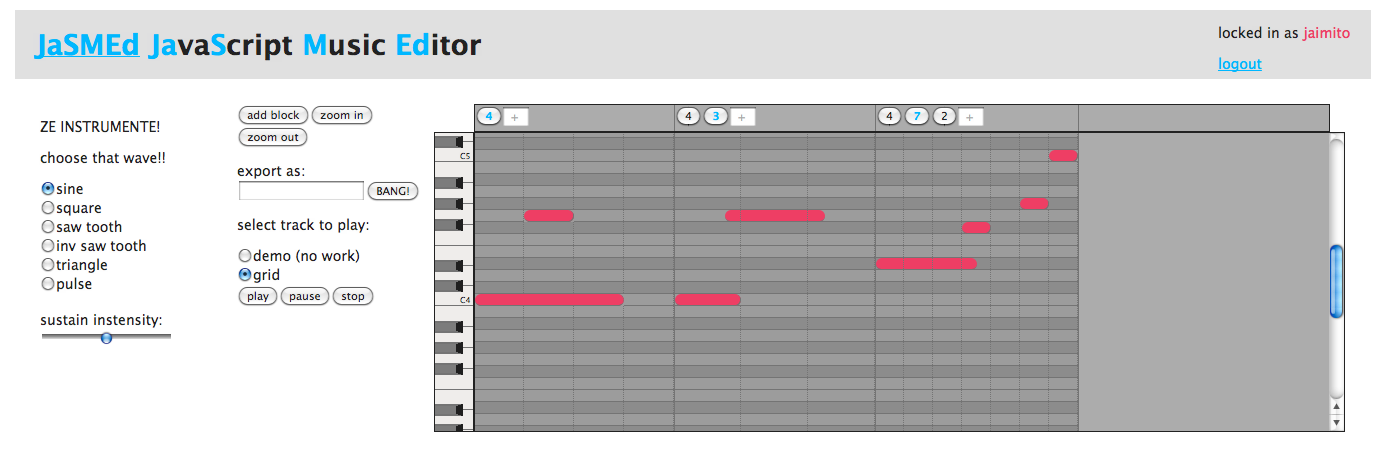
\includegraphics[width= \linewidth]{./track}

\subsection{Édition}
La partie édition représente une partition musicale à éditer/jouer, spécifiant la hauteur, la longueur, et la position de chaque note. L'éditeur permet la navigation verticale et horizontale : horizontalement sur l'axe du temps et verticalement selon la hauteur du son.\\
L'utilisateur peut faire défiler l'éditeur horizontalement en mettant son pointeur de souris près du bord d'un des blocs situés aux extrémités, ou verticalement avec la barre de défilement.

\medskip
On peut ajouter un layer à un bloc en entrant le nombre de subdivision voulu dans la zone rectangulaire (avec un +) au dessus de celui-ci.
On peut ensuite changer le layer apparent du bloc en cliquant sur le bouton correspondant.

\medskip
Pour créer une note qui aura la durée voulue, il faut d'abord sélectionner/créer le bon layer puis cliquer sur une case du bloc.
Il est possible de cliquer sur une case et relâcher la souris sur une case suivante de la même hauteur pour pouvoir créer une note plus longue.\\
Pour l'instant on ne peut pas supprimer de notes, pour commencer une nouvelle session il faut recharger la page.

\subsection{Lecture}
Les outils de lecture sont simplement constitués de trois boutons :
\begin{itemize}
\item play
\item pause
\item stop
\end{itemize}
    
\subsection{Outils}
L'utilisateur peut exporter son morceau sur le serveur (l'enregistrer) en lui donnant un nom dans la zone sous "export as", puis en appuyant sur le bouton "BANG!".
On peut agrandir ou rétrécir la taille des blocs dans la zone d'édition avec les boutons zoom in et zoom out.
Si on veut rajouter un bloc à notre piste on clique sur le bouton add block.
    
\subsection{Instrumentation}
Le panneau d'instrumentation permet de choisir le type de l'oscillateur qui jouera la piste lors de la lecture, ainsi que de modifier l'intensité du sustain de l'enveloppe ADSR en bougeant le slider.

\section{Conclusion}
Ce projet est une réussite du point de vue de l’expérience accumulée, avoir pu proposer et développer jasmed nous a permis de faire un pont entre notre master PSAR et l’intérêt que nous portons à l’informatique musicale. De plus, nous finissons notre M1 avec une connaissance plus précise des technologies internet actuelles, et une vision plus claire de la direction que prend le web : interactif et collaboratif.

Avec ce rapport nous avons souhaité fournir les clés et raccourcis au programmeur désirant développer une application audio sur le web. Ces informations accumulées pendant ce semestre lui permettront plus rapidement d’appréhender les erreurs à éviter avec HTML5.

Jasmed est un outil unique en son genre et nous comptons continuer à le développer et le laisser libre d’accès sur GitHub, il y a déjà des étudiants qui souhaitent rejoindre le projet.
Nous nous sommes efforcés de construire l’architecture de jasmed sur des bases saines, ce qui permet maintenant d’ajouter simplement de nouveaux modules, d’améliorer séparément ceux qui sont déjà existants, et de maintenir aisément un code bien commenté.

Améliorations futures :
Il est prévu de permettre à l’utilisateur d’éditer plusieurs instruments dans la même session, de lui laisser plus de choix quant à l’instrumentation, … //met on tout le futur envisagé ?


\begin{thebibliography}{99}

\bibitem{Flanagan}
  David Flanagan,
  \emph{JavaScript: The Definitive Guide}.
  \\O'Reilly,
  2011.

\bibitem{audiolib}
Jussi Kalliokosky,
\emph{Audio Library Application Programming Interface}.\\
\url{https://github.com/jussi-kalliokoski/audiolib.js}

\bibitem{draft}
W3C (,
\emph{Audio Library Application Programming Interface}.\\
\url{https://github.com/jussi-kalliokoski/audiolib.js}

\end{thebibliography}

\appendix

\section*{Diagramme de l'architecture}
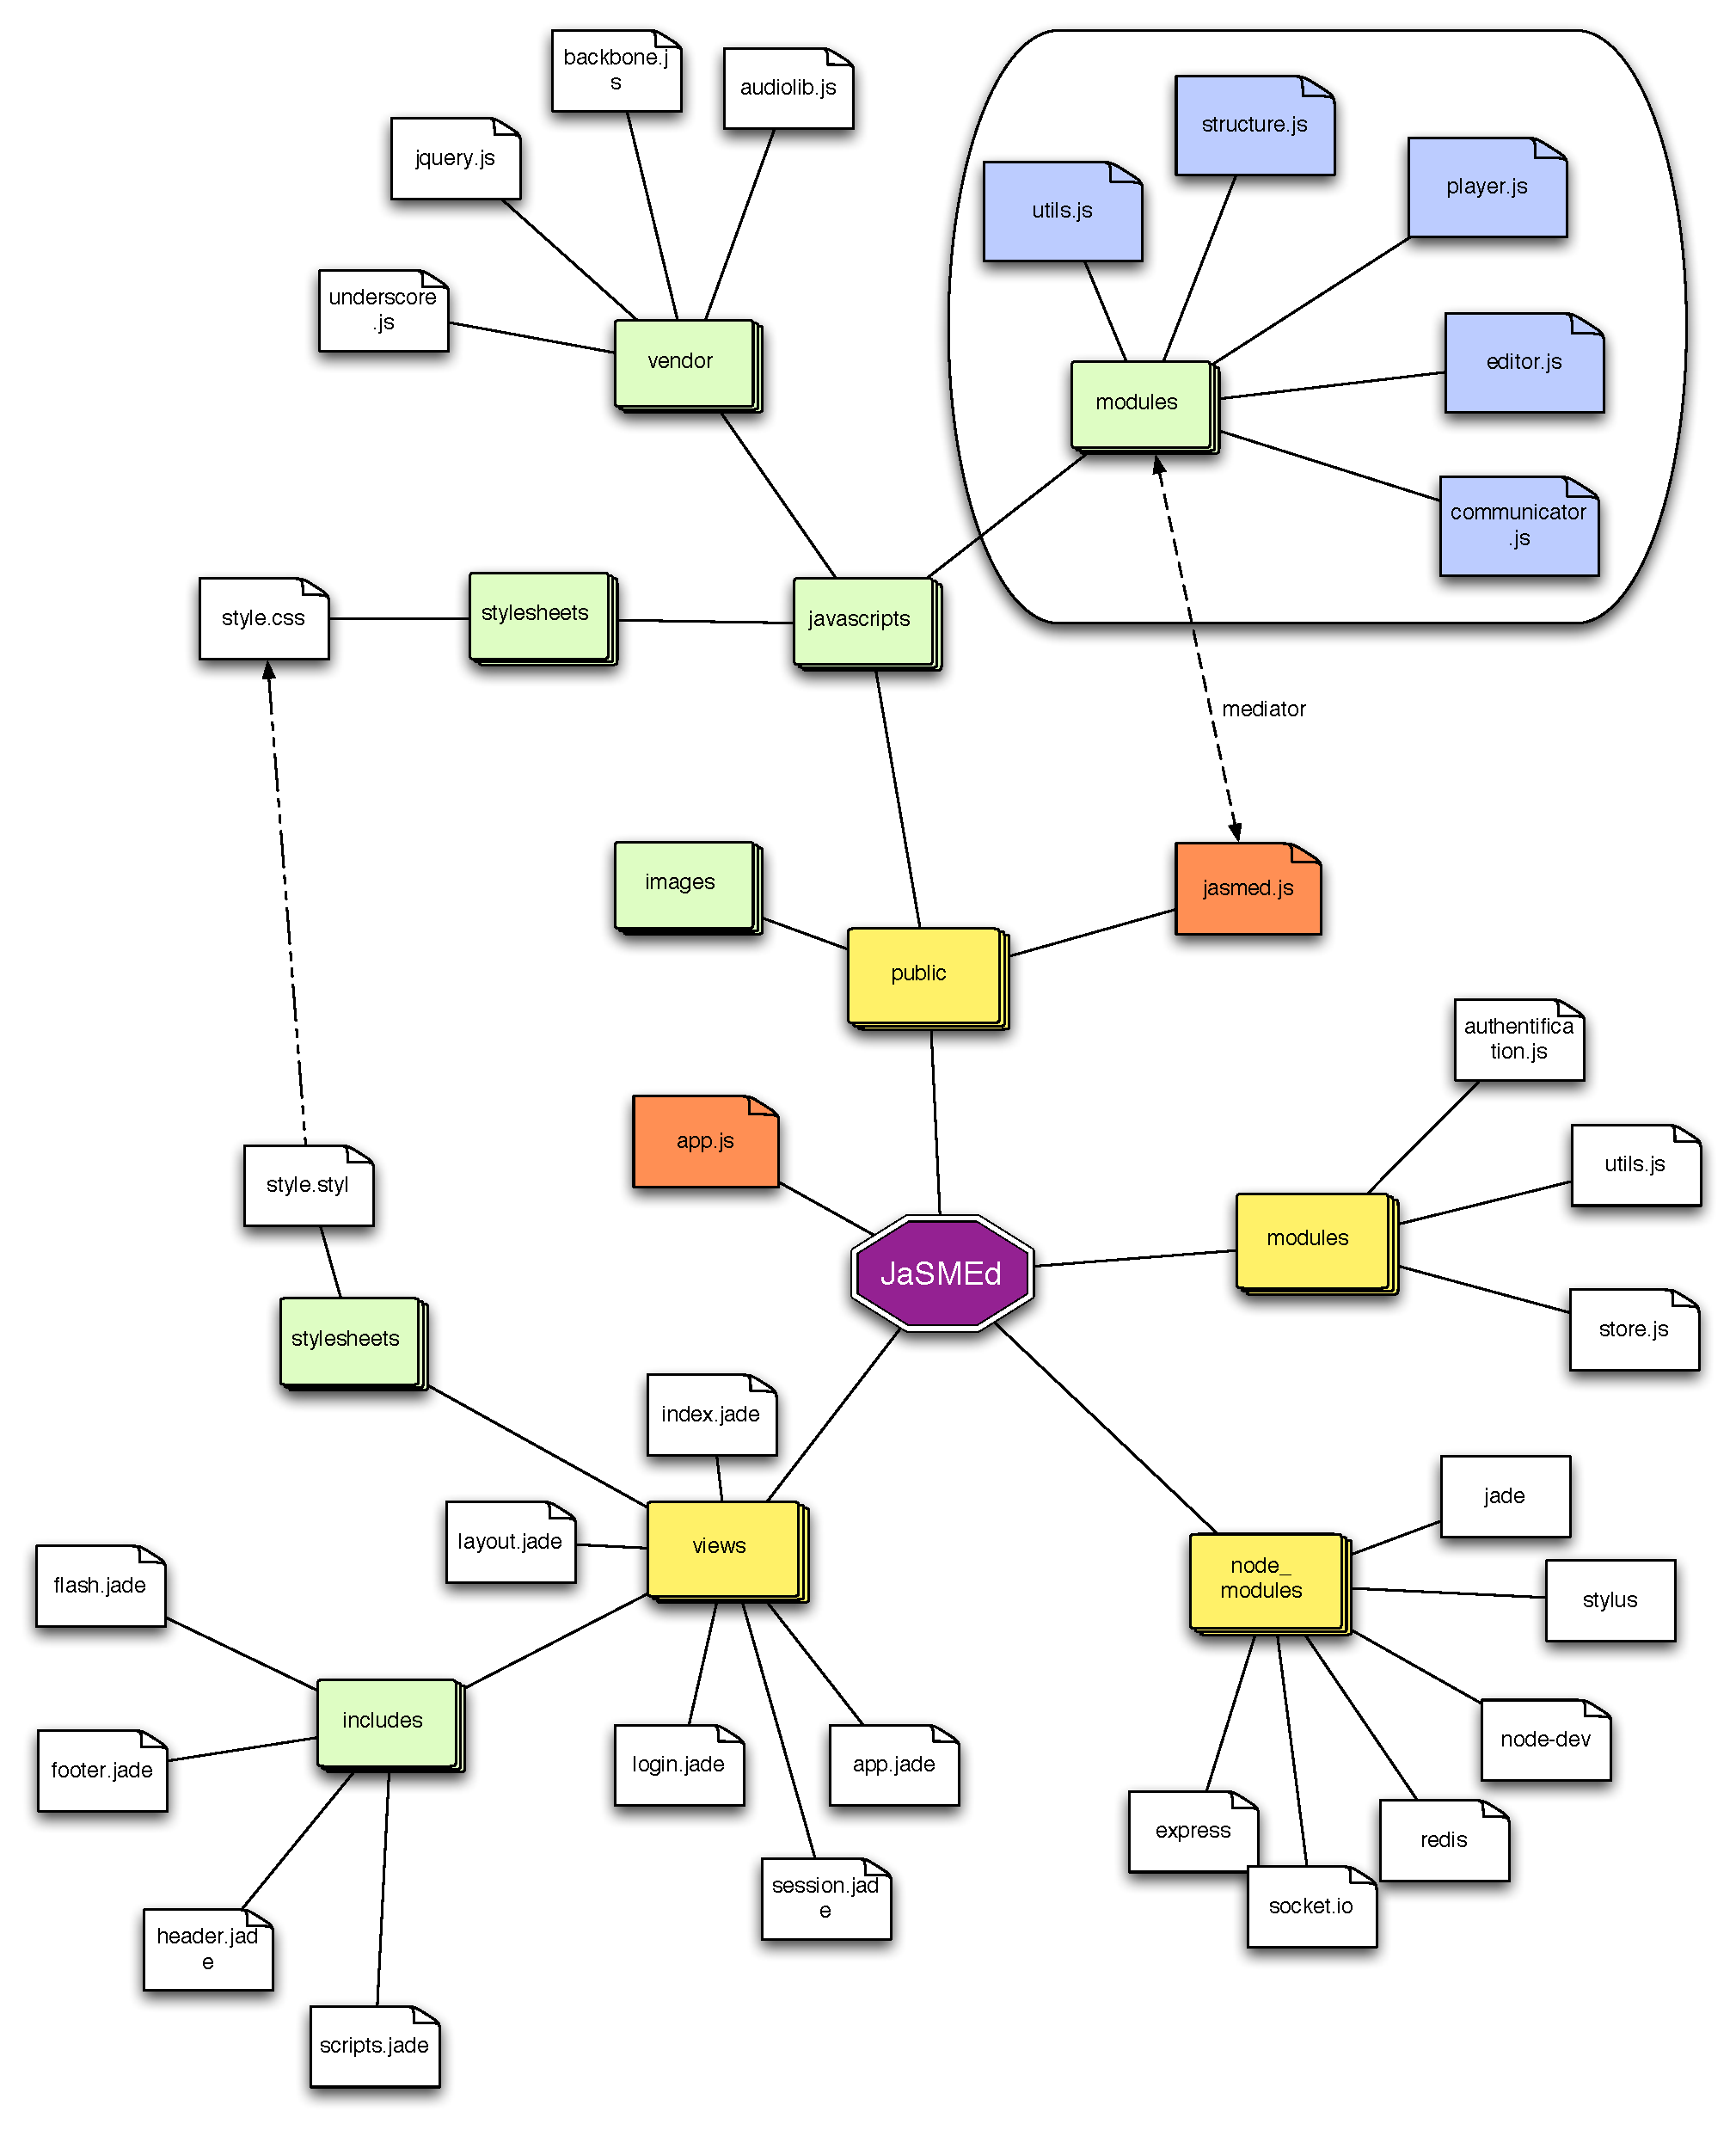
\includegraphics[width=\linewidth]{./jasmedDirectory}

\section*{Messages échangés}

\end{document}

pb et difficultés:
-MIDI (chap conception)
-largeur de bloc ->affichage non-cohérent, curseur de lecture
-sample décalage
-app scalable -> modulaire/gestion centralisé, MV*
-latence d'initialisation lecture